    \documentclass{article}
    \usepackage[margin=1in, top = .8in, left=.8in]{geometry}
    \usepackage{comment}
    \usepackage{amsmath, amssymb}
    \usepackage{framed}
    \usepackage{enumerate}
    \usepackage{comment}
    \usepackage{tikz,pgfplots}
    \usepgfplotslibrary{fillbetween}
    \pgfplotsset{compat=1.15}
    \usepackage[hyphens]{url}
    
    \newcommand{\fgraff}{
    \begin{minipage}[l][.30\textwidth]{3 in}{
    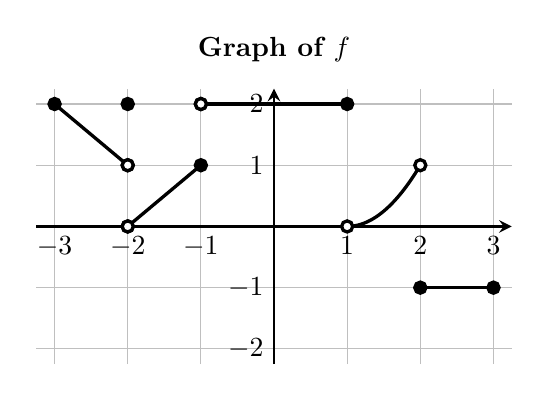
\begin{tikzpicture}
    \begin{axis}[
       	xmin=-3.25, xmax=3.25,
    	ymin=-2.25, ymax=2.25,
    	major tick length={0},
    	xtick={-3,-2,...,3}, ytick={-2,-1,...,2},
    	line width=1pt, title={\textbf{Graph of $f$}},
     	axis lines=center, height=2 in, width=3 in, grid=major,
     	restrict y to domain=-2.25:2.25
    	]
    	\addplot [mark=*, black, smooth, very thick] plot coordinates {(-3,2)(-2,1)};
    	\addplot [mark=*, black, smooth, very thick] plot coordinates {(-2,3)};
    	\addplot [mark=*, black, smooth, very thick] plot coordinates {(-2,0)(-1,1)};
    	\addplot [mark=*, black, smooth, very thick] plot coordinates {(-1,2)(1,2)};
    	\addplot [mark=*, black, smooth, very thick] plot coordinates {(2,-1)(3,-1)};
        \addplot [black, smooth, very thick, samples=100, domain=1:2] {(x-1)^2};
        \addplot [black, only marks, very thick, mark=*, mark options={scale=1, fill=white}]
        coordinates{(1,0) (2,1) (-1,2) (-2,1) (-2,0)};
        \addplot [black, only marks, very thick, mark=*] coordinates{(-2,2)};
    \end{axis}
    \end{tikzpicture}
    %\end{center}
    }
    \end{minipage}}
    
    \newcommand{\ggraff}{
    \begin{minipage}[l][.30\textwidth]{3 in}{
    %\begin{center}
    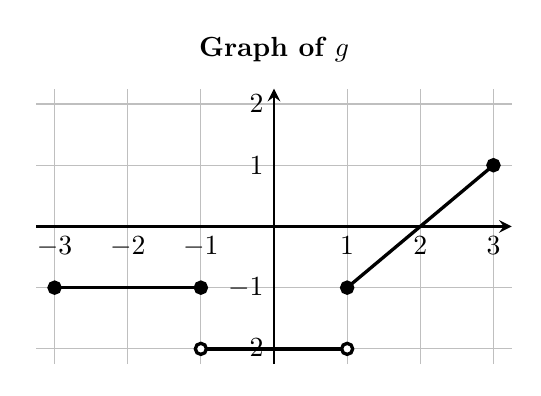
\begin{tikzpicture}
    \begin{axis}[
       	xmin=-3.25, xmax=3.25,
    	ymin=-2.25, ymax=2.25,
    	major tick length={0},
    	xtick={-3,-2,...,3}, ytick={-2,-1,...,2},
    	line width=1pt, title={\textbf{Graph of $g$}},
     	axis lines=center, height=2 in, width=3 in, grid=major,
     	restrict y to domain=-2.25:2.25
    	]
    	\addplot [mark=*, black, smooth, very thick] plot coordinates {(-3,-1)(-1,-1)};
    	\addplot [mark=*, black, smooth, very thick] plot coordinates {(1,-1)(3,1)};
    	\addplot [black, very thick, mark=*, mark options={scale=1, fill=white}] plot coordinates {(-1,-2)(1,-2)};
    \end{axis}
    \end{tikzpicture}
    %\end{center}
    }
    \end{minipage}}
    
    \begin{document}
    
    \begin{center}
        \large \textbf{Homework 2}
    \end{center}
        %\item[\textbf{Week 2}]
            \begin{itemize}
                %\item Sync (Week 1):
                \item Part 1
                    \begin{enumerate}
                        \item Using the laws of logarithms and properties of summations, show that $$\ln\left(\prod_{k=1}^n \frac{\lambda^{x_k}e^{-\lambda}}{x_k!}\right)=\ln(\lambda)\sum_{k=1}^n x_k -n\lambda - \sum_{k=1}^n \ln(x_k!)$$
                        \item Write down the first five terms of the sequence and find an explicit formula for the general term $a_n$.
                            \begin{enumerate}
                                \item An arithmetic sequence with a common difference of $3$ and the $10$th term is $41$
                                \item A geometric sequence with a common ratio of $\frac{1}{5}$ and the first term is $7$
                                \item $a_1=5$ and $a_n=3na_{n-1}$ for $n\geq 2$
                            \end{enumerate}
                        \item Evaluate each of the following sums.  These same sums will be seen again later in this course in the context of computing the area between a function and the $x$-axis.
                            \begin{enumerate}
                                \item $\displaystyle \sum_{j=1}^{10} \left(\frac{1}{5}j+4\right)$  (Note that your answer should be a positive numeric value.)
                                \item $\displaystyle \sum_{j=1}^{8} \frac{1}{2}\left[\left(1+\frac{j}{2} \right)^2 -4\left( 1+ \frac{j}{2}\right) + 5\right]$  (Note that your answer should be a positive numeric value.)
                                \item $\displaystyle \sum_{j=1}^{n} \frac{4}{n}\left[ \left(\frac{j}{n}\right)^2 - \frac{j}{n} + 1 \right]$  (Note that your answer should be an expression in the variable $n$.)
                            \end{enumerate}
                        \item Write the summation as an equivalent summation with the index of summation starting at $k=0$.
                            \begin{enumerate}
                                \item $\displaystyle \sum_{k=1}^n \frac{n!}{(k-1)!(n-k)!}p^k(1-p)^{n-k}$
                                \item $\displaystyle \sum_{k=4}^{98} 5\left(\frac{2}{3}\right) ^k$
                            \end{enumerate}
                        \item Evaluate each of the following sums.  Your answer should be an expression in the variable $m$.
                            \begin{enumerate}
                                \item $\displaystyle \sum_{k=5}^{m} (3k-4)$  (Hint: Consider reindexing to apply the formulas for special sums.)
                                \item $\displaystyle \sum_{k=2}^{m} (k^3+k^2)$  (Hint: Apply formulas for special sums and then subtract the extra value(s).)
                            \end{enumerate}
                        \item Let $f(x) = x^n$. Expand and simplify the expression $$\frac{f(x+h)-f(x)}{h}$$  Note that this rational expression for a function $f$ is called the \textbf{\em difference quotient} of $f$.  It will play a critical role a little later in the course.
                    \end{enumerate}
                %\item Async (Week 2):
                \item Part 2
                    \begin{enumerate}
                        \item Graph the piecewise function	     $$f(x) =  \begin{cases} 
                            8x-13-x^2 & \text{if $x \geq 3$} \\
                            -\ln{(4-x}) + 1 & \text{if $x < 3$} \\
                            \end{cases}$$
                            Hint: for the quadratic, try completing the square to find the vertex. For the log function, start by finding the domain.
                       \item Estimate $\displaystyle \lim_{x \rightarrow 1} \left(\frac{x}{x-1} - \frac{1}{\ln{x}}\right)$ numerically. Note: Even after the end of this week, we will still only have numerical techniques for solving this problem. However, using a technique called L'H\^{o}pital's Rule, in a few weeks we will have analytic methods for finding this limit.
                        \item Find the following limits:
                        \begin{enumerate}
                            \item   $\displaystyle \lim_{x \rightarrow 2^-} \frac{(x^2-4)(x^3-8)}{(x-2)^3}$
                            \item  $\displaystyle \lim_{h\rightarrow 0} \frac{(x+h)^2-x^2}{h}$
                            \item $\displaystyle \lim_{x\rightarrow 0} \frac{\left|x\right|}{x}$
                            \item $\displaystyle \lim_{x\rightarrow 0} \frac{\left|x^2\right|}{x^2}$
                            \item $\displaystyle \lim_{x \rightarrow 1} \frac{x^2-1}{|x-1|}$ (Hint: Try viewing it as a piecewise function, taking limits from the left and right separately. Graph it using technology to assure you have defined the function correctly.)
                            \item $\displaystyle \lim_{x \rightarrow 4} \frac{(x+4)(\sqrt{x}-2)}{x^3-64}$
                            \item Optional challenge: $\displaystyle \lim_{x \rightarrow 8} \frac{x-8}{\sqrt[3]{x}-2}$
                            \item Optional challenge: $\displaystyle \lim_{x \rightarrow 64} \frac{\sqrt{x}-8}{\sqrt[3]{x}-4}$
                        \end{enumerate}
                        \item By using numerical methods, and by drawing a graph of the function, guess the following limit:
                        $\displaystyle \lim_{x \rightarrow \infty} \frac{2x^2-3x}{x^2-3}$
                        \item The following limit questions are quite tricky. Be careful! For example, note that the limit laws only apply if all limits exist.
    
                        \begin{center}
                        \begin{tabular}{l r}
                        \fgraff & \ggraff
                        \end{tabular}
                        \end{center}
                        \begin{enumerate}
                        \item $\displaystyle \lim_{x\rightarrow -1} (f(x)+g(x))$
                        \item $\displaystyle \lim_{x\rightarrow -1} \frac{f(x)}{g(x)}$
                        \item $\displaystyle \lim_{x \rightarrow -2^-} g(f(x))$
                        \item $\displaystyle \lim_{x \rightarrow -2^+} g(f(x))$
                        \item $\displaystyle \lim_{x\rightarrow 1^-} f(g(x))$
                        \item $\displaystyle \lim_{x\rightarrow 2} \frac{f(x)}{g(x)}$
                        \end{enumerate}
    
    
                    \end{enumerate}
            \end{itemize}
    
    
    \end{document}
